\documentclass[11pt]{book}
%\usepackage{proceed2e}
\usepackage{naacl}
\usepackage[hyphens]{url}


%%%% Fill out all these macros
\newcommand{\thesisTitle}{Fake News Detection}
\newcommand{\authorName}{Mahsa Ghaderan}
\newcommand{\advisor}{Main Guardian}
\newcommand{\advisorTitle}{Professor Sauleh Eetemadi} % assistant, associate prof?
\newcommand{\advisorDepartment}{Computer Science and Engineering}


\newcommand{\readingCommitteeOne}{First Reader}
\newcommand{\readingCommitteeTwo}{Second Reader}
\newcommand{\graduationYear}{2021}


%\usepackage{} -- add any other packages you want
\usepackage{amsfonts}
\usepackage{multirow,tabularx}
\usepackage{listings}
\usepackage{makecell}
\usepackage[linesnumbered]{algorithm2e}
\usepackage{amssymb}
\usepackage{graphicx}
\usepackage{amsmath}
\usepackage{float}
\usepackage{fullpage}
\usepackage{mathrsfs}
\usepackage{subcaption}
\usepackage{hyperref}% http://ctan.org/pkg/hyperref
\hypersetup{%
  %colorlinks = true,
  linkcolor  = black
}
\usepackage{mdwlist}
\usepackage{xspace}
\usepackage{setspace}
\usepackage{times} % Set the typeface to Times Roman
\usepackage[scaled]{helvet} % ss
\usepackage{courier} % tt
\normalfont
\usepackage[T1]{fontenc}


%\usepackage[showframe=true]{geometry}
\usepackage{changepage}
\usepackage[labelfont=bf]{caption} % boldface caption title for floats
\usepackage[square]{natbib}
\usepackage{enumitem}
\usepackage{natbib}
\usepackage{array,multirow}
\usepackage{fixltx2e}
\usepackage{booktabs}
\usepackage{bbm}
\usepackage{soul}
\usepackage{relsize}
\usepackage{eso-pic}
\usepackage{xspace}
\usepackage{epsfig}
\usepackage{graphicx}
\usepackage{amsmath}
\usepackage{amssymb}
\usepackage{float}
\usepackage{multirow}
\usepackage{rotating}
\usepackage{balance}
\usepackage{wrapfig}
\usepackage{enumerate}
\usepackage{caption}
\usepackage{framed}
\usepackage{enumitem}
\usepackage{multirow}
\usepackage{graphicx}
\usepackage{color}
\usepackage{fixltx2e}
%\usepackage{tkz-graph}
\usepackage{caption}
\usepackage{subcaption}
\usepackage{mathtools}
\usepackage{pifont}
\usepackage{scrextend}
\usepackage{sidecap}
\usepackage{graphicx}
\usepackage{enumitem}

\usepackage{eqexpl}
\begin{document}

%% Replace all of the orange portions with your personal info

\begin{titlepage}
\begin{center}
\vspace*{\fill}
\singlespace
\thispagestyle{empty}
{\LARGE { \thesisTitle \\} %self-explanatory
\doublespacing
\vspace*{\baselineskip}
{\large \authorName }\\ %self-explanatory
\vspace*{1.5\baselineskip}
\large A Thesis
\\ submitted in partial fulfillment of the\\
requirements for the degree of\\
% \vspace*{\baselineskip}
‌Bachelor\\
\vspace{1.5\baselineskip}
% \begin{figure}[h]
%     \centering
%     
\includegraphics[width=3cm]{iust.jpeg}
% \end{figure}

Iran University of Science and Technology
\\ \graduationYear}\\ % add year in YYYY format (e.g. 2020)
\vspace{1.5\baselineskip}

%add reading committee (just the reading committee, not the supervisory committee):
\large \textit{Reading Committee:} \\

\ifdefined\secondAdvisor 
    \advisor, Co-Chair \\
    \secondAdvisor, Co-Chair \\
\else
    \advisor, Chair
\fi

\readingCommitteeOne \\

\ifdefined\readingCommitteeTwo
    \readingCommitteeTwo \\
\fi
    

\vspace{2\baselineskip}
  Program Authorized to Offer Degree: \\
Computer Engineering
  
% \newcommand{\advisor}{Main Guardian}
% % if you have two advisors, uncomment these two
% \newcommand{\firstAdvisor}{Parent One}
% \newcommand{\secondAdvisor}{Parent Two}
% \newcommand{\readingCommitteeOne}{First Reader}
% \newcommand{\readingCommitteeTwo}{Second Reader}

  
  
%%% Insert year and name:
  \vspace*{\fill}
  \clearpage
  \thispagestyle{empty}
  \singlespace{
  \copyright~Copyright \graduationYear \\ %add year in YYYY format (e.g. 2020)
  \vspace*{\baselineskip}
  \authorName} %self-explanatory
\end{center}
\end{titlepage}


\doublespacing

%% Replace all of the orange portions with your personal info

\thispagestyle{empty}
\begin{centering}
\vspace{1in}
Iran University of Science and Technology \\
\vspace*{1.\baselineskip}
{\bf Abstract}\\
\vspace*{1\baselineskip}

{\thesisTitle}\\ %self-explanatory
\vspace*{1.\baselineskip}
{\authorName} \\ %self-explanatory
\vspace*{1.\baselineskip}


\ifdefined\secondAdvisor
    Co-chairs
    \else
    Chair
\fi
of the Supervisory Committee:\\ %change to co-chair if co-advised 
\advisorTitle~\advisor\\ \vspace{-.5em} \advisorDepartment \\
\ifdefined\secondAdvisor
    \secondAdvisorTitle~\secondAdvisor\\\vspace{-.5em}\secondAdvisorDepartment \\
\fi
\end{centering}
\vspace*{\baselineskip}
These days increase in unauthenticated internet sources has led to spreading fake news vastly. Failure to detect misinformation promptly can have significantly irreparable damages on the walk of life. Recent researches have improved stance classification as a primitive step to detect fake news in English. Moreover, they have less focus on recognizing fake news. In this work, we have developed a deep learning model based on ParsBERT to improve the accuracy of the Persian stance classification. We over-sampled the available imbalanced dataset in Persian to compensate lack of data in such a low-resource language. Then, we implemented a model to detect fake news in Persian by using our best stance classifier and other manually extracted features. Consequently, we achieved an accuracy of 85\% for stance classification and 99\% for fake news detection on the employed dataset.

\bigbreak
\vspace*{3cm}
\bigbreak
Keywords: Machine Learning, Deep Learning, Natural Language Processing, BERT, Oversampling, Stance Classification, Fake News Detection

\chapter*{Acknowledgements}
%% self explanatory:

I want to give my warmest thanks to my supervisor, professor Sauleh Etemadi, Who made this project possible. He fully supports me and guides me. He also led me in each stage of writing and doing this report.  

Specially thanks to my mother, father, and my sister, who support me every single day of my life. They were motivating me in this way.

I am also thankful for my teammates and the friends Mr. Majid Zarharan, Mr. Mehdi Moghadami, Mr. Armin Gholami, and Miss Zahra Hosseini. They helped me to improve this project and giving me valuable advice. 

Finally, Thank God for letting me through all these hard days and give me such power to finish this work. I keep trusting you for my future. 
%% Replace all of the orange portions with your personal info

\clearpage

% if you need an extra blank page to make the dedications start on an odd number, then un-comment the following:
%%\clearpage\thispagestyle{empty}\mbox{}\clearpage 

\begin{center}
{\LARGE \textbf{DEDICATION}}
\hspace{0pt}
\vfill
{To {\color{orange}????}} %add whomever you want here
\vfill
\hspace{0pt}
\end{center}



\tableofcontents{}
\listoffigures
\listoftables
\clearpage

%\chapter {Background}
%
\section{BERT}
Pretrained language models have significant improve on many natural language model tasks such as natural language inference task (\cite{bert}). One of most impressive and powerful deep learning language model for text processing, is BERT which is stands for Bidirectional Encoder
Representations from Transformers (\cite{bert}) and developed by Google. And has received state of the art result due its previous researches (\cite{bert}). \cite{spotfake} improved its performance by make usage of the BERT language model in fake news detection. BERT base version contains 12 transformer blocks, containing 110 million parameters. There are also another variant of BERT such as large including 24 transformer blocks and multilingual BERT. BERT models are trained of Wikipedia corpus. 

One application of BERT is using first top layers of BERT model as contextual word embedding (\cite{book_datafake}). This model suggests a vector that representing a word which best fit in the current context.  BERT is a masked language model. It randomly masks some tokens and learn to predict masked tokens correctly. BERT utilizes bidirectional transformer, it means that BERT can inferred both left to right and right to left.

   
{\color{green}TODO}

\section{ALBERT}
{\color{green}TODO}

\section{ParsBERT}
{\color{green}TODO}

% \chapter {Literature Review}
% The major purpose of reviewing the literature is to determine what has already been done that relates to your topic. 
This section basically supports the background section by providing evidence for the proposed hypothesis.
describe all the studies that you have mentioned in the background section. 

present a more focused survey of the specific studies that are associated with the precise objective of your study.

learn more about the previous research published on the topic, and this eventually translates into literature review when you write your research paper.


{\color{orange}(book,chptr9,AlgorithmsCreate and PreventFakeNews)}
A research team 7 based at Canada’s Waterloo University broke down the fully
automated fact-checking process into four steps:
1. Retrieve documents relevant to the claim in question.
2. Determine the “stance” of each document, meaning
whether it supports, rejects, or is ambivalent/unrelated
to the claim.
3. Assign a credibility score to each document based on its
source.
4. Assign a truthfulness score to the claim by combining the
document stances weighted by the document credibility
scores (and highlight relevant facts/context from the
documents).

The first step can be a tricky one, because it is more open-ended than the matching step conducted by Full Fact, Logically, and Squash: rather than searching through a specific database of fact-checks for a match to the claim, one needs to scour the Web for any documents that might have information related to the claim. Google’s use of BERT to analyze the text in user search queries is bringing us closer to this task, but many challenges still remain.

The third step is essentially what Google and Facebook already do—through Google’s use of PageRank and human evaluators and through Facebook’s NEQ scores, as you saw in Chapters 6 and 8. 

The fourth step is straightforward once the first three are complete, so the Waterloo team decided to focus on

the second step—stance detection—to see how well that could be automated. They used a data set of fifty thousand articles to train a deep learning classification algorithm that looks at the body of each article and the headline of the article and estimates whether the body agrees with the headline, disagrees with it, discusses it without taking a stance, or is unrelated to the headline. Their algorithm scored a very respectable ninety percent accuracy, which was considerably higher than previous attempts by other researchers. 

The main insight in their work was to start with Facebook’s massive pre-trained deep learning algorithm RoBERTa and then do additional focused training to fine-tune the algorithm for the specific task at hand. This general process of fine-tuning a massive pre-trained deep learning algorithm is called “transfer learning,” and it has been an extremely successful method in AI, so it is not at all surprising that this is the right way to go when it comes to stance detection—it just wasn’t possible before BERT and RoBERTa came out.




{\color{orange}(book,chptr9,AlgorithmsCreate and PreventFakeNews)}
The Allen Institute for Artificial Intelligence (which you briefly encountered in Chapter 2 for its Grover system for detecting GPT-2 type generated text) developed a free tool called SciFact 8 to help with fact-checking medical claims related to COVID-19. The user types an assertion, or chooses from a list of suggestions, such as “Higher viral loads of SARS-CoV-2 are associated with more severe symptoms,” and a list of medical research publications is returned, each with an estimated score of how strongly it supports or rejects the assertion—similar to the Waterloo team’s stance detection—and a few potentially relevant excerpts from each publication are provided.

When I tried this higher viral load assertion, seven articles were returned, four supporting and three refuting—and while not all of them seemed relevant or accurately labeled, the results were enough to show that there is not a strong scientific consensus on this issue.

Their algorithm uses BERT to process text, and it was fine-tuned as follows. 

First, a modestly sized collection of medical publications was assembled and the citation sentences (i.e., sentences that include a citation to another research publication) were extracted. Next, human experts manually rewrote these sentences as medical assertions; they were allowed to use the text surrounding each citation sentence, but not the paper being cited. The human experts also created negated versions of these assertions, so that the algorithm would have examples of assertions refuted by the literature, not just ones supported by it. They then went through by hand and decided
whether each assertion is indeed supported by the article it cites, or refuted by it, or whether there is insufficient information to make this decision—and in the cases where it was labeled as supported or refuted, the experts highlighted the passages in the article’s abstract that provided the strongest basis for this label. 

Roughly speaking, this process is how they trained their BERT-based algorithm to do all three tasks involved: retrieve articles relevant
to a given assertion, estimate the stance of each article in relation to the assertion, and extract relevant passages from each article’s abstract. 
The researchers’ framework in principle applies to all kinds of medical and scientific assertions—not just COVID-related ones—but since training their algorithm involves careful manual work with the data, they decided to launch this tool initially in a limited setting and scope. The reader is cautioned, and the researchers readily admit, that this tool is largely intended to show what is possible and what challenges remain, rather than to be blindly trusted. They tested a few dozen COVID-19 assertions and found the algorithm returned relevant papers and correctly identified their stance about two-thirds of the time. While this tool should not replace finding and reading papers manually, it might still help with a quick first-pass assessment of medical claims.


%\chapter {Introduction}
%These days, fake news and false information have been vastly flooding the Internet by numerous not verified news agencies with aims ranging from affecting individual people’s beliefs and decisions to influencing major events such as political elections (\cite{memory_network}). As days go by, the importance of detecting stance automatically is appealing more attention. Insofar as it has been suggested that automatic stance detection is the first step towards assisting human fact checkers to detect inaccurate claims \cite{UCLMR}.


%these notions by Claire Wardle from First Draft, 2 misinformation is “unintentional mistakes such as inaccurate photo captions, dates, statistics, translations, or when satire is taken seriously.”, and disinformation is “fabricated or deliberately manipulated audio/visual context, and also intentionally created conspiracy theories or rumours.”.\cite{stace_survey}

The purpose of automatic stance detection is to find the type of a relation between specified sentences against a given text by utilizing machines. So it is possible to evaluate what is the orientation of a news source towards a particular issue \cite{UCLMR}. The selected sentence could be a claim, a news item, an idea, a social network post, or any other source. Also, the text could be retrieved from news agencies, weblogs, posts that are shared on social media, and any other available text. Choosing the source and context of sentences and texts depends on the goal of the defined task. Four considered labels are \textit{Agree}, \textit{Disagreed}, \textit{Discussed}, and \textit{Not Enough Information}. 

Gathering a sufficient amount of data is a vital step to achieve reliable predictor model. Both number of records in the dataset and the quality of each sample have a significant effect on prediction accuracy. \cite{takestancefake}) gathered fifty thousand articles-headline pairs for their dataset, and achieved a respectable ninety percent accuracy, which was considerably higher than previous attempts by other researchers (\cite{book_fake}). Though, in some contexts, there isn't enough available data. Here is where transfer learning methods play a vital role and compensate lack of data. We pre-trained a model on a large text corpus in a general context and then fine-tune the model on task-specified data. \cite{takestancefake} used RoBERTa model which is pre-trained on Facebook data. Then fine-tune it on the specific task at hand.
Also, \cite{stance_robust} improved its accuracy by fine-tuning BERT model.

Researchers have suggested various methods for stance classification. One cluster of methods mainly focuses on deep learning approaches. The precision of models is improved by using word embeddings such as BERT, using recurrent neural networks such as LSTM, BiLSTM (\cite{stanceCI}), and utlizing attention-based network (\cite{stanceCI}). Besides, novel model architectures such as Memory Network (\cite{memory_network}), are currently proposed.

One possible way of evaluating the veracity of a given claim is detecting the stance of that claim against available trusted sources. Stance detection task traditionally were used in political and ideological debates fields \citep{stance_robust}. The idea of using Stance Detection techniques to analyze news items correctness has become caught researchers attention since 2016. Consistency of a sentence through sources can be retrieved by stance detection methods. Consequently, stance detection can be considered as a subtask of fake news detection (\cite{book_datafake}), and It is easier to judge a claim by its stance against other sources. So estimating the stance of a particular claim against available documents can be the first step in detecting fake news. 


%\chapter {Fact Verification and Extraction}
%\label{chapter:two}
%

\section{Literature Review}
Overview previous works and papers.
\section{Introduction}

\section{Experiments}
ParsFEVER Code + Another paper codes and mutations on that code. 
\section{Results}
\section{Conclusion}

% If you are copying and pasting material from one of your papers, then remember to:
% \begin{itemize}
%     \item Remove the abstract and instead add a little overview of the chapter and how it ties in to the rest of the thesis. You should also mention the original paper's source like: ``This chapter includes materials originally published in $\backslash$citet\{myownppr\}''
%     \item Make sure the formatting still works -- this is single column now!
%     \item Consider rephrasing conference-paper-style language:
%     \begin{itemize}
%         \item Find every place you mention some variation of ``in this paper'' and say ``in this chapter'' instead.
%         \item Remove or rephrase the parts where you talk about ``our main contributions''.
%         \item Rephrase the language describing code and data releases.
%     \end{itemize}
%     \item Replace the conclusion section with a summary section. Again, you should tie this chapter back to the main themes of the thesis.
% \end{itemize}



% \begin{wrapfigure}{r}{0.3\textwidth}
%     \centering
%     \includegraphics[width=.3\textwidth]{example-image-b}
%     \caption[Short title for wrapfigure]{You can also make inline figures.}
%     \label{chap2:fig:ex2}
% \end{wrapfigure}

% Here are a few notes about the layout and usage of this latex template:

% \paragraph{Captions} In order for the captions from figures and tables to show up cleanly in the lists of figures and tables, you should use the caption command with the bracket argument to create a short title for the list of figures/tables, like:

% \texttt{$\backslash$caption [shortened title]\{full caption\}}

% \noindent as in Figure~\ref{chap2:fig:ex} and Table~\ref{chap2:tab:ex}.

% \paragraph{Citations} This latex was given to me with an old NAACL style file that uses the standard \texttt{$\backslash$citep}  and \texttt{$\backslash$citet}  commands as in Table~\ref{chap2:tab:ex}.  I don't think it supports \texttt{$\backslash$cite} or \texttt{$\backslash$newcite}. Feel free to add commands as needed for you.

% \begin{figure}[tb]
%     \centering
%     \includegraphics[width=.5\textwidth]{example-image-a}
%     \caption[Short title  - only appears in list of figures]{Full caption, make it as long as you want.}
%     \label{chap2:fig:ex}
% \end{figure}


% \begin{table}[tb]
%     \centering
%     \begin{tabular}{lll}
%     \toprule
%          Latex command & Citation\\
%     \midrule
%         $\backslash$citep example & \citep{grice1975logic} \\
%         $\backslash$citet example & \citet{grice1975logic} \\
%     \bottomrule
%     \end{tabular}
%     \caption[Citation examples]{The style files that come included in this latex template use $\backslash$citep and $\backslash$citet.} 
%     \label{chap2:tab:ex}
% \end{table}

\chapter{Stance Detection}
\label{chapter:three}


\section{Preprocessing}
The first and mandatory preprocessing step is to tokenize words in the corpus in order to remove and detect special words. Four different following tokenizer performance on Persian language has been evaluated are Hazm, NLTK, Stanza, and BERT. 


After tokenization, a list of punctuation and Persian stop-words are considered as \textit{denied} and will remove from the corpus in this step. Firstly, the same stop-words was used which have been used by \cite{stance_persian}. After reviewing preprocessed corpus, it was hard to infer the stance from text pieces. So we chose stop-words carefully in a way not to lose refuting or supporting expressions. Kharazi\footnote{\label{fn:kharazi}github.com/kharazi/persian-stopwords} has classified Persian stop-words into verbal, nonverbal, and short. Verbs carry valuable information in news. Nonverbal stop-word class is a better choice to remove low-value words in this task. Besides adding and removing some words in news fields are evaluated against Kharazi's\footref{fn:kharazi} gathered stop-words. 

Also English number characters will remove from the corpus before tokenizing. After preprocessing tokens, all tokens will be concatenated with a space character and considered as prepossessed and clean corpus.


\section{Word Representation}
{\color{green} TODO}
To represent a corpus, tokens should be converts to vectors. Good vectors have to carry semantic of each word or n-grams, sequential words contents, and be as brief as possible. As a baseline three different Bag-of-word (\cite{bow}), TF-iDF (\cite{tfidf}), and Word-to-Vector (\cite{word2vec}) algorithms are evaluated against each other. More details are explained below.

\section{Features}
\label{sec:features}
In machine learning algorithms, feature engineering can be considered the most important step because the desired model trains patterns only corresponding to predictors. Extracting sufficient predictors as compact as possible to having the best predicting accuracy and time-efficient	, requires numerous trials and errors. In the following part of this section, extracted features are explained in detail.
\subsection{Similarity}
The similarity score is offered by \cite{stance_persian}. This feature calculates how much a claim is similar to a headline or a news article, depends on the task. Three following sequence matching score is considered for this feature by utilizing \textit{difflib}\footnote{docs.python.org/3/library/difflib.html} python library.

\begin{itemize}
	\item Ratio: Similarity score in float range 0,1. This parameters calculates from equation \ref{eq_ratio}
	\begin{equation}
		\label{eq_ratio}
		ratio = \frac{2.0 * M}{T}
	\end{equation}
	where:
	\begin{eqexpl}[25mm]
		\item{$T$}Number of elements in both sequences.
		\item{$M$}Number of matches.
	\end{eqexpl}
	\item Quick Ratio: This parameter estimates an upper bound on the Ratio.
	\item Real Quick Ratio: This parameter estimates an upper bound on the Ratio.
\end{itemize}
\subsection{Root Distance}
This feature is suggested by \cite{stance_persian}. Root Distance stands for the distance between the root of a headline and some collected hedge, refuting and reporting words. Firstly, a set of words considered as mentioned group are gathered, and then for each word distance is calculated.
%\newline{\color{red}=================TODO========================}
\subsection{ImportantWords}
List of a controversial and challenging words in news  gathered by \cite{stance_persian} and considered as \textit{important-words}. This feature is a zero-based list with the length of important words, and each cell stands for one word in \textit{important-words}. The list carries the number of repetitions of desire words in a specific news article.
\subsection{Is Question}
Is-Question identifies whether a claim or headline of a news article ends with question marks or not. \cite{stance_persian} dataset contains a column dedicated to this feature.
\subsection{Has Two Parts}
Has-Two-Parts is if a claim is constructed of two separate parts. \cite{stance_persian} dataset contains a column dedicated to this feature.
\subsection{Polarity}  
The polarity of a text can be utilized in a variety of tasks. This feature presents how positive or negative a text is. Different algorithms are developed to predict the polarity of a text. In this project, \cite{persent} dataset is used to calculate each sample sentiment. \cite{persent} contains a dictionary of words with their sentiment score between -1 and 1. The more negative the word meaning, the lower its polarity point. For each word presents in each sample at most first 30 nonzero polarity value saves in a zero initialed vector with 30 lengths. As \cite{persent} contains only 1500 word polarity values, it can't cover all words in corpus and it has a far way to improve. 

In this project, an idea is applied to extend PerSent (\cite{persent}) polarity dataset is to use a language model. It is possible to predict similar words with a particular word and estimate their similarity score with a language model. Firstly, similar words that don't polarity score in PerSent with their similarity scores extract from a pre-trained language model. Then search each word in the PerSent dataset (\cite{persent}) and apply equation \ref{eq_polar} average through all similar words polarity scores, to estimate the desired word polarity score.

\begin{equation}
	\label{eq_polar}
	polarity\_score\left(w\right) = \frac{\Sigma_{w^{`} \in W} Similatiry\left(w^{`}, w\right) . Polarity\left(w^{`}\right)}{\Sigma_{w^{`} \in W} Similatiry\left(w^{`}, w\right)}
\end{equation}

where: 
\begin{eqexpl}[25mm]
	\item{$w$}Desire word $\notin$ PerSent datast.
	\item{$W$}Similar words, Predicted by the language model
	\item{$Similarity$}Similarity score for 2 words which is predicted by the language model.
	\item{$polarity$} Polaroty score which is estimated by \cite{persent} dataset.
\end{eqexpl}

\bigbreak
One alternative is to use a deep neural networks model to predict score polarity of a word whether word-level or sentence-level. But due to the lack of a Persian dataset in news context, it is not practical. Available datasets for sentiment analysis are mainly gathered from customer comments on special businesses. For instance \cite{polar_hotel} used 2 different datasets, first it translated English sentiment analysis corpus and second used comments on hotels. \cite{polar_servic} used dataset from SnappFood\footnote{snappfood.ir}, DigiKala\footnote{digikala.ir} comments. One main problem with these datasets is the different use of language between user comments and news. Users mostly use everyday language on the other hand news agencies use formal language.

\section{Machine Learning}
Machine learning algorithms aim to learn patterns on a corpus of data while training procedure, then predict classes of news articles test data by those patterns (\cite{book_fake}). Machine learning algorithms have powerful performance even in complex problems. In comparison to deep learning models, Machine learning algorithms learn patterns according to their fed manually extracted predictors, and we don't have any other choice rather than relying on those number of extracted predictors (\cite{book_fake}). So extracting useful features  is a critical step in machine learning. The more meaningful and suitable predictors they see for a task, the better patterns they can find during the training procedure. Figure \ref{fig:mlschm} illustrates a basic schematic of each machine learning models. The description of each predictor described in detail at section \ref{sec:features}, is evaluated by following machine learning methods.   

\begin{figure}% 
	\centering
	{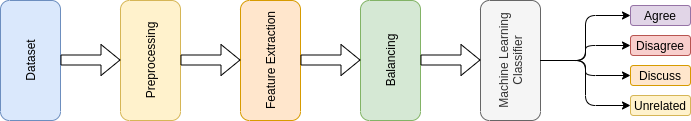
\includegraphics[width=14.5cm]{statistics/schema/ml.png} }
	\caption{Schematic of each machine learning model.}%
	\label{fig:mlschm}%
\end{figure}

\section{Balancing}
As mentioned in section \nameref{sec:dataset}, Figure \ref{fig:datacom}, the number of samples in dataset classes was imbalanced. As a result, models bias on majority class and there may not enough sample in minority class for a model to learn that, this leads to having high accuracy score (Equation \ref{eq:acc}) while having low f1 score (Equation \ref{eq:f1}).  

\bigbreak
There are several algorithms to deal with imbalanced datasets. In \cite{stance_persian} minority class forms only 7.4\% of data (Figure \ref{fig:datacom}). So it's not practical to rely on only one method and except to perform in the best way. Consequently, three different methods were used in this project in order to deal with this phenomenon. Methods of balancing a dataset which is used in this project are described in the following sections.  
	
\subsection{Extending dataset}
The simplest method is to gather data for classes except for the majority class. But unfortunately, it is not always practicable. Another way of extending a dataset is to use another existing dataset which has similar gathering logic and it is possible to map these two dataset classes. 

ParsFEVER (\cite{parsfever}) is a Persian dataset set based on FEVER (\cite{fever}) dataset is gathered for fact extraction and verification task. \cite{parsfever} claims are generated from Wikipedia\footnote{wikipedia.org} articles manually, then pieces of evidence for each claim are extracted from Wikipedia separately by distinct annotators. This dataset contains three \textit{Support}, \textit{Refute}, and \textit{Not Enough Info} classes. 
\begin{itemize}
	\item {\color{green!70!black}\textbf{Support:}} The article obviously proves the given claim. 
	\item {\color{red!60!black}\textbf{Refute:}} The article obviously disproves the given claim.
	\item {\color{gray}\textbf{Not Enough Info:}} There isn't enough information in the article about the claim. 
\end{itemize}                

According to Figure \ref{fig:datacom} two \textit{Agree} and \textit{Disagree} class in \cite{stance_persian} dataset suffers from lack of samples. In this project, \textit{Supports} and \textit{Refutes} samples from \cite{parsfever} dataset are mapped to \textit{Agree} and \textit{Disagree} class of \cite{stance_persian} dataset respectively. 
But it is not possible to extend \textit{Discuss} or \textit{Unrelated} class by ParsFEVER, because they are both merged in \textit{Not Enough Info} class. As a result, two \textit{Agree} and \textit{Disagree} extended as much as possible with random selected samples from ParsFEVER dataset. Sample distribution is illustrated in figure \ref{fig:datab1}. Dataset is still imbalanced in one class for both Article to Claim and Headline to Claim.

\begin{figure}%
	\centering
	\subfloat[\centering Artcile to Claim]{{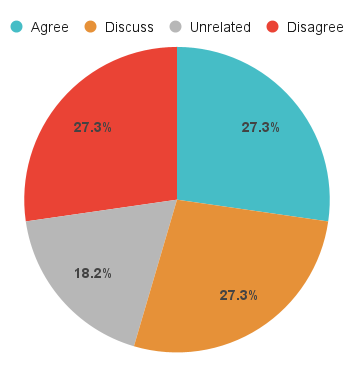
\includegraphics[width=6cm]{statistics/stance/a2c_b1.png} }}%
	\qquad
	\subfloat[\centering Headline to claim ]{{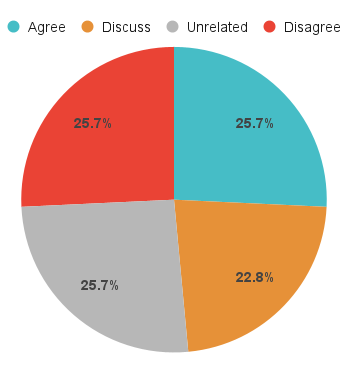
\includegraphics[width=6cm]{statistics/stance/h2c_b1.png} }}%
	\caption{Comparison between Article to claim and Headline to claim labels, samples distribution in \cite{stance_persian} dataset, after extending by \cite{parsfever} .}%
	\label{fig:datab1}%
\end{figure}

\subsection{Oversampling and Undersampling}
 
All mentioned oversampling methods are evaluated against each other in this project and utilized from oversampling package of \textit{imblearn} \footnote{imbalanced-learn.org/stable/references/over\_sampling.html} python library. 

\subsection{Tune mode parameters}
 The last but not least important balancing method is to choose a robust learning algorithm for an imbalanced dataset, Choosing a weight of each class according to the ratio of samples of each class and choosing an optimizer and loss function that can overcome an imbalanced dataset. After applying previous methods to balance the dataset, this step can be skipped in this project. 




\section{Deep Learning}
In deep learning approach, a combination of all predictors can be fed into the model and the model on its own will automatically learns which predictor is useful for the task. This property is the biggest advance of deep learning in comparison to machine learning (\cite{book_datafake}). In contrary, in machine learning it was a critical step to design input predictors that the model can performs the best. And hours of trying different combination of predictors is needed (\cite{book_fake}). \cite{stance_robust} assessed that, In contrast deep learning models, machine learning models that is trained on a single dataset, usually generalize poorly to other domains.
The schematic of deep learning model is shown in figure \ref{fig:dlschm}. Headline-to-claim and Article-to-claim models have same schematic. Only some parameters vary in each model. In the following sections, pretrained language model used for stance detection are described. 
\begin{figure}% 
	\centering
	{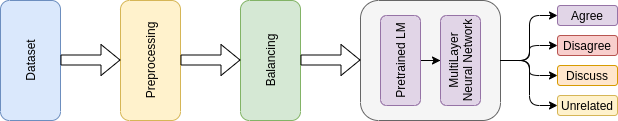
\includegraphics[width=14.5cm]{statistics/schema/dl.png} }
	\caption{Schematic of each deep learning model.}%
	\label{fig:dlschm}%
\end{figure}


\section{Article to Claim}
Deep learning models perform far better on language inference tasks so they are better choices for article-to-claim stance classification. To calculate stance of a claim toward the body of a news, three different model based on a pre-trained Persian language model based on BERT, ParsBERT, and  ALBERT are evaluated against each other. 

\section{Fake News Detection}
	\label{sec:fakenews}
Shematic of fake news pipeline is shown in figure \ref{fig:fnschm}. To detect a news article veracity, headline-to-claim and article-to-claim stance detection models, are considered as a black box. Four news articles is considered to evaluate veracity of a claim. Firstly, stance of a claim toward each headline of desired news articles and the body of the news article predict by stance classifier models. All predicted stance vectors are concatenated and along with some other features are fed into a multi-layer perception network in order to predict the claim veracity.

\begin{figure}% 
	\centering
	{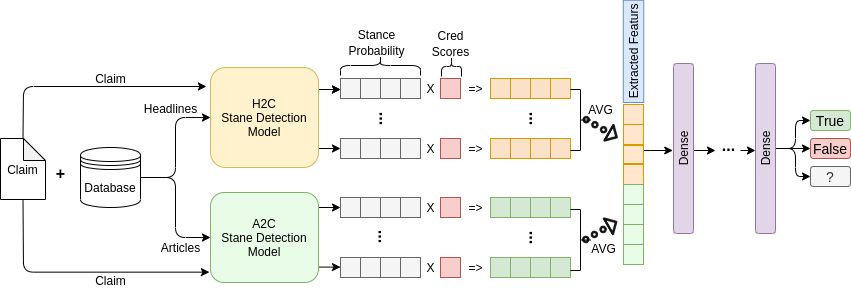
\includegraphics[width=14.5cm]{statistics/schema/fn.png} }
	\caption{Schematic of each fake news detection model.}%
	\label{fig:fnschm}%
\end{figure}

Credibility of news websites is one of the most important extracted feature. The credibility can be calculated through the following steps (The credibility score of head-claim and article-claim is calculated similarly except using their related stance ground truth):

\begin{itemize}
	\item \textbf{Initialization}: The credibility score of all news websites that are existing in the \cite{stance_persian} dataset is set to zero at first. For the test set or predicting new samples, if the website doesn't exist in the data set, credit score is set to 0.1.


	\item \textbf{Quantification:}
	For each sample in the dataset, credibility score changes according to Table \ref{tbl:cred}. $\rho$ value is calculated from equation \ref{eq:cred} if it is needed.
	\begin{table}[H]
		\centering
		\caption{Value of credibility according to GroundTruth and Veracity labels. }
		\setlength{\extrarowheight}{5pt}%
		\begin{tabular}{|l|l|l|}
			\hline
			GroundTruth & Veracity & Value \\
			\hline \hline
			Agree       & True     & $+1$    \\
			\hline
			Disagree    & False    & $+1$    \\
			\hline
			Agree       & False    & $-1$    \\
			\hline
			Disagree    & True     & $-1$    \\
			\hline
			Discuss     & True     & $+\rho$    \\
			\hline
			Discuss     & False    & $-\rho$   \\
			\hline
			Unrelated     & -   & No change   \\
			\hline
			-     & Discuss    & No change   \\
			\hline
		\end{tabular}
		\label{tbl:cred}
	\end{table}

	\begin{equation}
	\label{eq:cred}
	\rho = \frac{P(x,Agree) - P(x,Disagree)}{P(x,Agree) + P(x,Disagree)}\\
	\end{equation}

where: 
\begin{eqexpl}[25mm]
\item{$P(x,Agree)$} Probability of Agree
\item{$P(x,Disagree)$} Probability of Disagree 
\end{eqexpl}
	
	\item \textbf{Score Calculation:} The credibility score for each news website is calculated from equation \ref{eq:honesty}.
	\begin{equation}
	\label{eq:honesty}
	H(X) = \frac{\sum_{i=1}^{k_{X}} credibility\,of\,x_{i}}{k_{X}}
	\end{equation} 
	where:
	\begin{eqexpl}[25mm]
		\item{$X$} A news website
		\item{$k_{x}$} The number of news article in the dataset from x
		\item{$credibility\,of\,x_{i}$} Due to table \ref{tbl:cred}
	\end{eqexpl}

\end{itemize}


Also another features are extracted to detect fake news, such as :
\begin{itemize}
	\item One-hot encoding of the news website domain
	\item The ratio of samples that have been properly labeled as agree or disagree to the total sample of the news website (Correct ratio)
	\item The ratio of samples that have been wrongly labeled as agree or disagree to the total sample of the news website (Wrong ratio)
	\item The ratio of the total number of news website articles to the total number of articles in the data set.	
\end{itemize}





\chapter {Fake News}
\label{chapter:four}
\section{Literature Review}
\section{Introduction}
\section{Experiments}
Ideas and works inorder to detect fake news.
\section{Results}
\section{Conclusion}


\chapter{Conclusion}
Machine learning models are evaluated on Persian stance detection task as baseline. Multiple predictors are extracted and different combination of them are applied on machine learning models to find out the most effective predictor combination. Due imbalanced samples distribution in the \cite{stance_persian} dataset, extending the dataset by ParsBERT dataset (\cite{parsbert}) and oversampling methods are discussed and compared to each other.

In the Persian stance detection task, using deep language models boosts performance noticeably. BERT and ParsBERT as it's alternative have high ability to make inference from a given content so they can represent current content sufficiently and test accuracy in the model based on ParsBERT language model is equal to 85.48\%. As the result,  BERT language models predict stance detection 10\% higher than machine learning algorithm on average. In contrast, requires time consuming feature engineering and parameter tuning and they can't achieve high accuracy on language inference tasks. For both machine learning and deep learning models performance decrease on article-to-claim task. Despite of this issue, machine learning algorithm have achieve even higher than 70\% accuracy score on headline-to-claim task. The black-box nature of machine learning algorithms means that nobody really knows why an AI lie detection system works as it does, nor what it is actually doing (\cite{book_fake}). 

The best pretrained stance detection model on headline-to-claim and article-to-claim are separately utilized in fake news detection. We have achieve 99\% accuracy score on the \cite{stance_persian} dataset. Though, number of samples in the dataset gathered by \cite{stance_persian} contains 1624 samples. Increasing number of samples help model to improves model generalization.

Adding attention layers to the classifier have improve results in current researches. Fox instance, \cite{book_disinformation} alleged that using attention layers in the model have make a great contribution on accuracy scores. Utilizing such models can also make increase on the ability of these models to go beyond the current state in such low-resource settings. Besides, increasing number of samples in the \cite{stance_persian} dataset toward achieving balanced dataset can help the model to distinguish each class precisely. 
 
 
 

\bibliography{main.bib}	
\bibliographystyle{acl_natbib}

% Optionally: add appendices
\newpage
\newcommand{\beginsupplement}{%
    \setcounter{chapter}{0}
    \renewcommand{\thechapter}{\Alph{chapter}}%
 }

\beginsupplement
\chapter{Appendix One}
\section{Appendix section 1}
\begin{table}[]
    \centering
    \begin{tabular}{c|c}
         &  \\
         & 
    \end{tabular}
    \caption{Table in the Appendix}
    \label{tab:my_label}
\end{table}

\end{document}

% you're all done, congrats!